Dabiskā valodas apstrāde (NLP -- \textit{natural language processing}) ir starpdisciplināra datorlingvistikas un mākslīgā intelekta nozare, kas strādā pie tā, lai datori varētu saprast cilvēka dabiskās valodas ievadi. Dabiskās valodas pēc būtības ir sarežģītas, un daudzi NLP uzdevumi ir slikti piemēroti matemātiski precīziem algoritmiskajiem risinājumiem. Palielinoties korpusu (liela apjoma rakstītas vai runātas dabiskās valodas kolekcija) pieejamībai, NLP uzdevumi arvien biežāk un efektīvāk tiek risināti ar mašīnmācīšanās modeļiem \cite{nlp2018}. Dabiskās valodas apstrādei ir liels biznesa potenciāls, jo tas ļauj uzņēmumiem palielināt peļņu samazinot izdevumus, no kuriem lielākais parasti ir darbs. %\% pakalpojumu nozares uzņēmumu izdevumi ir darbs. Var minēt tech layoffs, specifically, Meta’s Year of Efficiency


Viens no svarīgākajiem korpusiem tieši nodomu noteikšanā ir aviokompāniju ceļojumu informācijas sistēmu (ATIS -- \textit{Airline Travel Information Systems}) datu kopa. Tā ir audioierakstu un manuālu transkriptu datu kopa, kas sastāv no cilvēku sarunām ar automatizētām aviolīniju ceļojumu informācijas sistēmām. ATIS datu kopa nodrošina lielu ziņojumu un ar tiem saistīto nodomu skaitu, ko plaši izmanto kā novērtējuma (\textit{benchmark}) datu kopu klasifikatoru apmācībai nodomu noteikšanā \cite{atis1990}.

Lielo teksta korpusu un mašīnmācīšanās modeļu precizitātes vēsture ir cieši saistīta. Agrīnie mašīnmācīšanās algoritmi balstījās uz nelielām manuāli veidotām datu kopām, kas ierobežoja to efektivitāti. Viens no pirmajiem korpusiem bija \textit{Standard Sample of Present-Day American English}, plašāk pazīstams kā \textit{The Brown Corpus}, kas tika izdots 1964-1965. gadā un sastāvēja no apmēram viena miljona vārdu angļu teksta no dažādiem avotiem \cite{brown-corpus}, tas ir mazs apjoms teksta salīdzinot ar mūsdienās pieejamo.

Procesoru jaudas palielināšanās kopā ar datoru un interneta savienojuma pieejamību plašākai sabiedrībai ir radījuši labvēlīgu vidi izveidot un uzglabāt lielu daudzumu digitālo datu, tostarp teksta formā. Lieliem teksta korpusiem ir bijusi izšķiroša loma efektīvu mašīnmācīšanās modeļu izstrādē. Mašīnmācīšanās modeļu efektivitāte ir proporcionāla tiem pieejamo apmācības datu lielumam un kvalitātei. %source

Pirms lielu teksta korpusu pieejamības mašīnmācīšanās modeļi aprobežojās ar mazām un salīdzinoši vienkāršām datu kopām, tādēļ bija grūti sasniegt augstu precizitāti dabiskās valodas apstrādes uzdevumos. Mūsdienās lielos teksta korpusos kā Common Crawl un Wikipedia ir miljardiem vārdu vairākās valodās, kas ļauj modeļiem iemācīties ģenerēt cilvēkiem līdzīgu valodu.




SNIPS -- \textit{Spoken Natural Language Interaction for Personal Assistant}) datu kopā ir 16 000 ievadi, kas sadalīti septiņos nodomos: SearchCreativeWork, GetWeather, BookRestaurant, PlayMusic, AddToPlaylist, RateBook, SearchScreeningEvent.








Three tasks are successively performed. Intent Classification consists in extracting the intent expressed in the query (e.g. SetTemperature or SwitchLightOn). Once the intent is known, Slot Filling aims to extract the slots, i.e. the values of the entities present in the query. Finally, Entity Resolution focuses on built-in entities, such as date and times, durations, temperatures, for which Snips provides an extra resolution step. It basically transforms entity values such as "tomorrow evening" into formatted values such as "2018-04-19 19:00:00 +00:00". Snippet 1 illustrates a typical output of the NLU component



Behind every chatbot and voice assistant lies a common piece of technology: Natural Language Understanding (NLU). Anytime a user interacts with an AI using natural language, their words need to be translated into a machine-readable description of what they meant. The NLU engine first detects what the intention of the user is (a.k.a. intent), then extracts the parameters (called slots) of the query. The developer can then use this to determine the appropriate action or response.


Natural Language Understanding (NLU) is a fundamental technology that powers chatbots and voice assistants. When a user communicates with an AI using natural language, the words are translated into a machine-readable format to determine what the user intended to convey. The NLU engine identifies the user's intent, followed by the extraction of parameters or slots of the query. By utilizing this extracted information, developers can determine the most suitable response or action to take.


he main metric used in this benchmark is the average F1-score of intent classification
and slot filling. The data consists in three corpora. Two of the corpora were extracted from
StackExchange, one from a Telegram chatbot. The exact same splits as in the original paper were
used for the Ubuntu and Web Applications corpora. At the date we ran the evaluation, the train and
test splits were not explicit for the Chatbot dataset (although they were added later on). In that case,
we ran a 5-fold cross-validation. T


Kad cilvēks ievada tekstu dabiskā valodā, tas tiek pārveidots jēdzientelpā. Pēc tam klasifikators nosaka lietotāja nodomu.

Dabisko valodu saprašanas (Natural Language Understanding (NLU)) uzdevumi iedalās divās daļās: nodomu noteikšana un parametru (slots) iegūšana no ievadiem.


% Table generated by Excel2LaTeX from sheet 'slots'
\begin{table}[htbp]
  \centering
  \caption{Add caption}
    \begin{tabular}{rlr}
    Intent Name &  Slots & Samples \\
          & \textcolor[rgb]{ .439,  .188,  .627}{ region} & Is it \textcolor[rgb]{ 1,  .753,  0}{cloudy} in \textcolor[rgb]{ 1,  0,  0}{Germany} right now? \\
          & \textcolor[rgb]{ 1,  0,  0}{ country} & Is \textcolor[rgb]{ .439,  .188,  .627}{South Carolina} expected to be sunny in 2 hours? \\
    ForecastCondition & \textcolor[rgb]{ .573,  .816,  .314}{ datetime} & Is there \textcolor[rgb]{ 1,  .753,  0}{snow} in Paris? \\
          & \textcolor[rgb]{ 0,  .69,  .941}{ locality} & Should I expect a \textcolor[rgb]{ 1,  .753,  0}{storm} near Mount Rushmore? \\
          & \textcolor[rgb]{ 1,  .753,  0}{ condition} &  \\
          & \textcolor[rgb]{ .929,  .49,  .192}{ point of interest} &  \\
    \end{tabular}%
  \label{tab:slots}%
\end{table}%








% pievieno info par NLU datasets un common crawl 100

Taču vai visas valodas ir līdzvērtīgi pārstāvētas korpusos? Viegli iztēloties, ka tādi lielie korpusi kā Common Crawl (kopš 2008. gada ievākti petabaiti datu no interneta mājaslapām, tostarp Vikipēdijas un Reddit) līdzvērtīgi pārstāv visu Zemes iedzīvotāju valodas. Taču valodu reprezentācija korpusos ir saistīta ar rakstītā teksta datu pieejamību šajā valodā, un neprecīzi atspoguļo cilvēku skaitu, kuri runā šajā valodā. Piemēram, valodai, kurā runā liels skaits cilvēku, korpusā var būt maz marķieru, ja šajā valodā ir maz digitāli pieejama rakstīta teksta.

Tomēr dažādi faktori traucē visiem rakstīt tekstus internetā, kas vēlāk nokļūst korpusos, piemēram, rakstītneprasme, nabadzība, ierīču un interneta nepieejamība, karš utml. Tā rezultātā korpusos ir disproporcionāli pārstāvēti gados jaunāku lietotāju no attīstītajām valstīm drukāti teksti, piemēram, GPT-2 apmācības dati tika ievākti no Reddit, un pēc Pew Internet Research pētījuma 67\% Reddit lietotāju Amerikas Savienotajās Valstīs ir vīrieši un 64\% vecumā no 18 līdz 29 gadiem.\cite{bender2021}.

Līdzīgi 87\% Vikipēdijas ierakstu veicēji ir vīrieši. Gandrīz puse dzīvo Eiropā un viena piektā daļa Ziemeļamerikā, salīdzinot ar 9.7\% un 4.8\% pasaules iedzīvotāju \cite{wikimedia2020}. Analizējot labojumus Vikipēdijas rakstos no 2001. līdz 2010. gadam, 1\% visbiežākie ierakstu veicēji uzrakstīja 77\% satura \cite{1percent}.

Korpusos tam ir vairākas praktiskas implikācijas gan sintaksē, gan semantikā. Piemēram, Vikipēdijas autors Brians Hendersons (\textit{Bryan Henderson}) 15 gados veica 90 tūkstošus labojumu, kur lielākā daļa izmaiņu ir no "comprised of" uz "comprised", kaut gan abas formas tiek pieņemtas un citos rakstiskos avotos "comprised of" ir izplatītāks (\ref{fig:distributed-representation} attēls). Tāpat BERT biežāk asociē cilvēkus ar invaliditāti ar negatīva sentimenta vārdiem un vairāki darbi to sasaista ar treniņu datu kopu īpašībām \cite{bender2021}. Pētīt negatīvu sentimentu valodu korpusos ir svarīgi, jo kompānijas reputācija ciestu, virtuālajam asistentam sniedzot atbildes ar negatīviem steriotipiem klientu apkalpošanas jomā.


\begin{figure}[h]
  \centering
  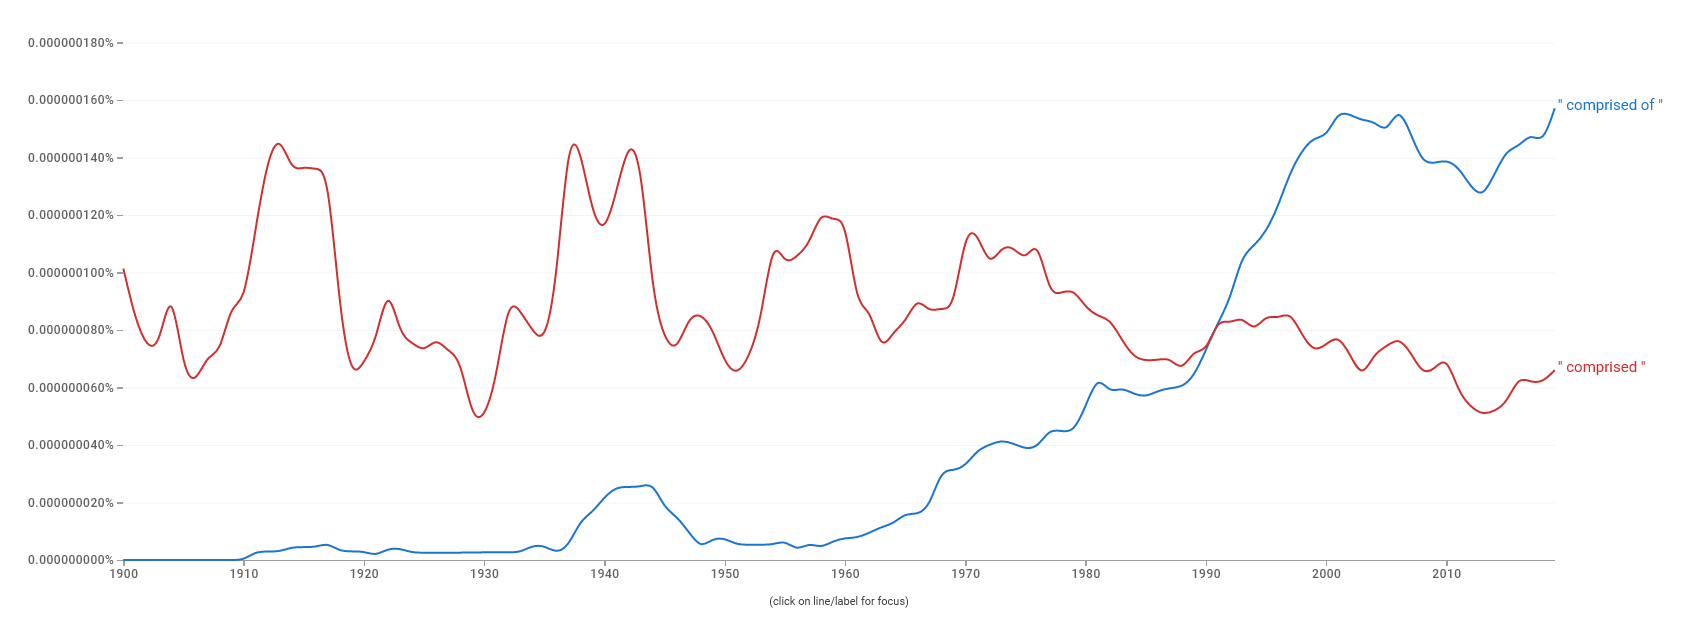
\includegraphics[width=\textwidth]{figures/comprised.png}
  \caption{Uz x ass attēloti gadi, uz y ass -- cik procentu no visiem vārdiem, kas ietverti angļu valodā rakstīto grāmatu korpusā (English 2019), ir "comprised of" un "comprised"? \cite{ngram-viewer}}
  \label{fig:comprised}
\end{figure}

Ar to tiek pierādīts, ka tekstu nav radījuši nejauši izvēlēta izlase cilvēku, tāpēc teksts nav neitrāls. Tiek paredzēts, ka virtuālos asistentus izmantos plašāks cilvēku loks nekā šobrīd internetā publicēto tekstu autori, tāpēc ir svarīgi, lai treniņdatos ir atbilstoši pārstāvēta potenciālo lietotāju valoda. 


Latviešu marķieru daļa Common Crawl 100 korpusā ir atkarīga no daudziem faktoriem, tostarp latviešu satura daudzuma tīmeklī un korpusa konstruēšanā izmantotās izlases metodikas. Iespējams, ka latviešu teksta saturs korpusā ir pārāk vai nepietiekami pārstāvēts, salīdzinot ar tā izplatību tīmeklī vai proporcionāli latviešu valodā runājošo īpatsvaram.


Kas padara valodu par maz-resursu? Mazāks skaits vārdu un teikumu datu kopās, tātad mazāks skaits tokenu uz kuriem trenēt daudzvalodu jēdzientelpu modeli. Piemēram, Common Crawl-100 korpusā, uz kura trenēts XLM-R modelis, svahili un urdu valodās ir 275M un 730M tokenu attiecīgi, darbā izmantotajās - lietuviešu, latviešu, igauņu - ir 1835M, 1198M un 843M tokenu attiecīgi (\ref{tab:cc-100} tabula), tātad šīs datukopas kontekstā tās var uzskatīt par maz-resursu. 


% Table generated by Excel2LaTeX from sheet 'cc-100'
\begin{table}[htbp]
  \centering
  \caption{Common Crawl-100 valodas un statistika: valodu saraksts ar marķieru (\textit{tokens}) skaitu (miljonos) un datu izmēru gibibaitos (GiB) katrai valodai}
    \begin{tabular}{llrr} \toprule
    ISO kods &  Valoda & Marķieri (M) & Izmērs (GiB) \\\midrule
    en    &  angļu & 55608 & 300.8 \\
    ru    &  krievu & 23408 & 278.0 \\
    lt    &  lietuviešu & 1835  & 13.7 \\
    lv    &  latviešu & 1198  & 8.8 \\
    et    &  igauņu & 843   & 6.1 \\
    ur    &  urdu & 730   & 5.7 \\
    sw    &  svahili & 275   & 1.6 \\\bottomrule
    \end{tabular}
  \label{tab:cc-100}
\end{table}

\begin{figure}[h]
  \centering
  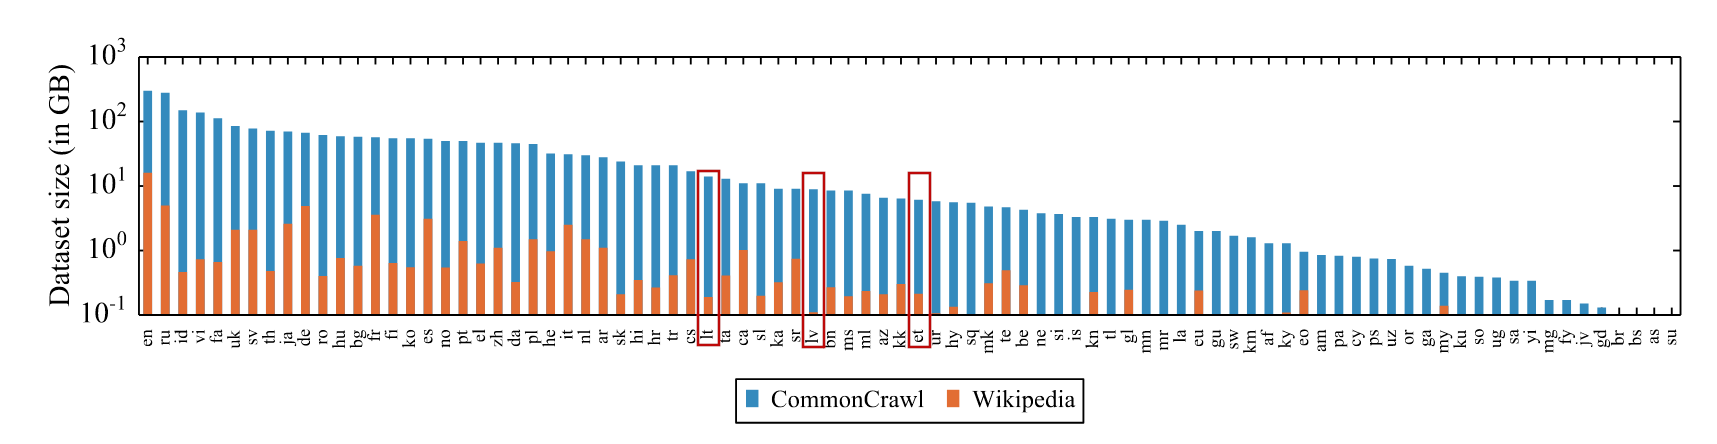
\includegraphics[width=\textwidth]{figures/dataset-size.png}
  \caption{Datu apjoms GiB (logaritmiskā skalā) valodām Wiki-100 korpusā, ko izmanto mBERT un XLM-100, un Common Crawl-100, ko izmanto XLM-R. Common Crawl-100 palielina datu apjomu par vairākām kārtām, jo īpaši maz-resursu valodās (lietuviešu, latviešu, igauņu valodas ar sarkanu izdalīju es) \cite{conneau2020}}
  \label{fig:dataset-size}
\end{figure}
